\section{Evaluatie}
\label{sec:eva}

\subsection{Resultaten}

\subsubsection{DV1: Beste classificatiemethode}
Het beste resultaat werd bereikt met Support Vector Machines gebruikmakend van \textit{stochastic gradient descent learning} en Elasticnet regularisatie. De features waren hierbij gestemd, met unigrams, bigrams en trigrams. Geen features zijn hierin weggelaten door minimale of maximale documentfrequenties. \par
Tabel \ref{tab:classrapport} laat de scores zien per partij met het aantal documenten in de test set. De $F_1$ scores per partij liggen tussen de 0.7 en 0.8. De one-issuepartijen, 50PLUS en PvdD, hebben scores daarboven, terwijl de coalitiepartijen, VVD en PvdA, lagere scores hebben. Figuur \ref{fig:confusionmatrix} laat zien waar de fouten in deze classificatie zitten. De meest karakteristieke features per partij zijn te zien in tabel \ref{tab:MostImportantWords}. Hierin is te zien dat vrijwel alle woorden verwijzen naar de partij of een Kamerlid van die partij.\par

\begin{table}[H]
\caption{Classificatie scores per partij van beste classificatiemethode (SVM). Gemiddelde van vijf iteraties.}
\label{tab:classrapport}
\centering
\begin{tabular}{lrrrlr}
\toprule
{} &  Precision &  Recall &  F1\_score & Accuracy &  Documenten \\
\midrule
50PLUS       &       0.97 &    0.85 &      0.91 &        - &        71.4 \\
CDA          &       0.80 &    0.79 &      0.80 &        - &       379.6 \\
ChristenUnie &       0.83 &    0.76 &      0.79 &        - &       215.4 \\
D66          &       0.78 &    0.75 &      0.76 &        - &       381.8 \\
GroenLinks   &       0.89 &    0.73 &      0.80 &        - &       209.2 \\
PVV          &       0.82 &    0.88 &      0.85 &        - &       345.0 \\
PvdA         &       0.72 &    0.71 &      0.71 &        - &       377.4 \\
PvdD         &       0.86 &    0.87 &      0.86 &        - &        81.2 \\
SGP          &       0.87 &    0.84 &      0.86 &        - &       134.8 \\
SP           &       0.73 &    0.85 &      0.78 &        - &       453.2 \\
VVD          &       0.77 &    0.73 &      0.75 &        - &       331.0 \\
Totaal       &       0.79 &    0.79 &      0.79 &     0.79 &      2980.0 \\
\bottomrule
\end{tabular}

\end{table}


\begin{figure}[H]
  \centering
    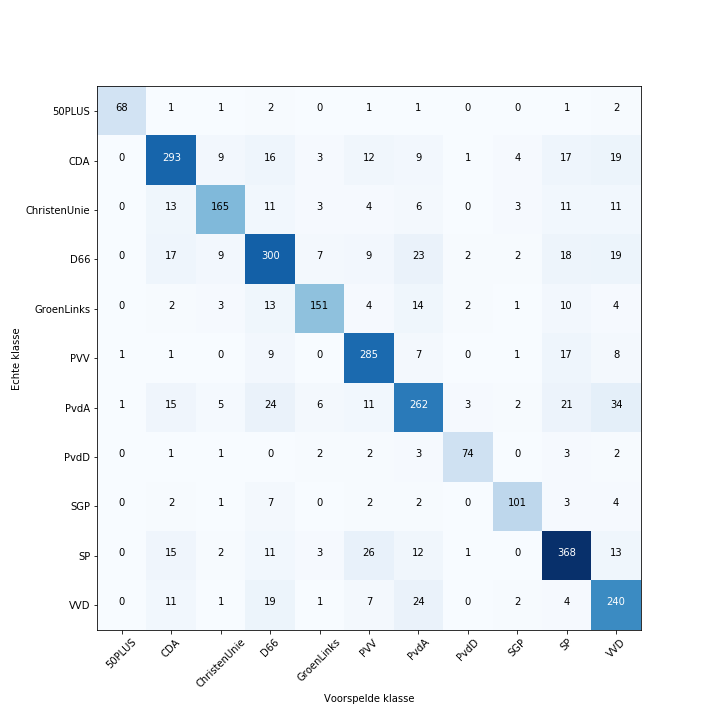
\includegraphics[width=0.60\paperwidth]{Verslag/Tables/confusionmatrix.png}
\caption{Confusion matrix van beste classificatie.}
\label{fig:confusionmatrix}
\end{figure}



\begin{table}[H]
\caption{Meest karakteristieke n-grams per partij op basis van beste classificatie gedurende kabinet-Rutte II.}

\label{tab:MostImportantWords} 
\centering
\hspace*{-1in}
\begin{tabular}{lllll}
\toprule
          50PLUS &               CDA &         ChristenUnie &                  D66 &          GroenLinks \\
\midrule
          50plus &               cda &      de christenunie &                  d66 &          groenlinks \\
   lid krol naar &           het cda &         christenunie &         mijn fractie &    lid van tongeren \\
    het lid krol &            de cda &        lid dik faber &  leden van veldhoven &   lid voortman naar \\
        lid krol &       cda fractie &          het lid dik &       lid van meenen &    het lid voortman \\
   krol naar mij &    de cda fractie &              lid dik &        van veldhoven &        lid voortman \\
       krol naar &       lid omtzigt &            dik faber &            veldhoven &            voortman \\
            krol &   het lid omtzigt &                faber &    lid van veldhoven &            tongeren \\
      van 50plus &  lid omtzigt naar &     leden voordewind &         leden schouw &        van tongeren \\
 gepensioneerden &      omtzigt naar &  de leden voordewind &      de leden schouw &  leden van tongeren \\
         ouderen &  omtzigt naar mij &                  dik &               d66 is &   de leden voortman \\
\bottomrule
\end{tabular}
 
\end{table} 
\addtocounter{table}{-1} 
\begin{table}[H]
\caption{Meest karakteristieke n-grams per partij op basis van beste classificatie gedurende kabinet-Rutte II. \emph{(Vervolg)}} 
\centering
\hspace*{-1in}
\begin{tabular}{llllll}
\toprule
              PVV &             PvdA &              PvdD &              SGP &             SP &             VVD \\
\midrule
              pvv &          de pvda &      lid ouwehand &              sgp &             sp &          de vvd \\
           de pvv &             pvda &  lid ouwehand nar &           de sgp &          de sp &             vvd \\
      islamitisch &    de partij van &  het lid ouwehand &      sgp fractie &   lid van gerv &  de vvd fractie \\
        lid graus &    van de arbeid &      ouwehand nar &   de sgp fractie &     sp fractie &     vvd fractie \\
    het lid graus &        de arbeid &  ouwehand nar mij &     led dijkgraf &  de sp fractie &       de vvd is \\
    lid graus nar &    partij van de &          ouwehand &  de led dijkgraf &   van gerv nar &          vvd is \\
          miljard &       partij van &       vor de dier &      led van der &       gerv nar &      vor de vvd \\
    graus nar mij &     pvda fractie &           de dier &  de led bisschop &   gerv nar mij &      wat de vvd \\
        graus nar &           arbeid &              dier &     led bisschop &           gerv &     vvd betreft \\
 madlener nar mij &  de pvda fractie &     de partij vor &           sgp is &       van gerv &  de vvd betreft \\
\bottomrule
\end{tabular}
 
\end{table}

\subsubsection{DV2: Invloed van namen}
In tabel \ref{tab:MostImportantWords} was al te zien dat de meest karakteristieke woorden voornamelijk bestaan uit partijnamen en namen van Kamerleden. In tabel \ref{tab:rapportwithoutnames} zijn de scores te zien van classificatie met partijnamen en namen van Kamerleden vervangen. Deze zijn aanzienlijk lager dan de scores uit deelvraag 1. In tabel \ref{tab:MostImportantWordsWithoutNames} is vervolgens te zien welke woorden het meest karakteristiek zijn per partij voor deze classificatie.\par
\begin{table}[H]
\caption{Classificatie scores per partij van beste classificatie zonder namen van Kamerleden of partijnamen.}
\label{tab:rapportwithoutnames}
\centering
\begin{tabular}{lrrrr}
\toprule
{} &  Precision &  Recall &  F1\_score &  Documenten \\
Partij       &            &         &           &             \\
\midrule
50PLUS       &      0.658 &   0.454 &     0.524 &        76.2 \\
   CDA       &      0.492 &   0.418 &     0.446 &       370.8 \\
ChristenUnie &      0.516 &   0.322 &     0.384 &       218.8 \\
   D66       &      0.502 &   0.434 &     0.452 &       377.2 \\
  GroenLinks &      0.486 &   0.338 &     0.368 &       210.8 \\
   PVV       &      0.512 &   0.768 &     0.612 &       349.8 \\
  PvdA       &      0.440 &   0.408 &     0.412 &       360.0 \\
  PvdD       &      0.554 &   0.596 &     0.572 &        89.0 \\
   SGP       &      0.592 &   0.660 &     0.620 &       134.8 \\
    SP       &      0.534 &   0.546 &     0.540 &       454.2 \\
   VVD       &      0.436 &   0.442 &     0.430 &       338.4 \\
 avg / total &      0.502 &   0.486 &     0.480 &      2980.0 \\
\bottomrule
\end{tabular}

\end{table}

\begin{table}[H] 
\caption{Meest relevante woorden per partij op basis van classificatie uit deelvraag 1 zonder partijnamen of namen van Kamerleden gedurende kabinet-Rutte II.} 
\label{tab:MostImportantWordsWithoutNames} 
\centering
\hspace*{-1in}
\begin{tabular}{lllll}
\toprule
                 50PLUS &             CDA &   ChristenUnie &           D66 &              GroenLinks \\
\midrule
        gepensioneerden &  PARTIJ fractie &   mensenhandel &  mijn fractie &                     zou \\
                ouderen &        inwoners &         zullen &          mijn &       kamer hierover te \\
                 oudere &          PARTIJ &       gezinnen &       fractie &     belastingontwijking \\
 koopkrachtontwikkeling &        regering &      inderdaad &    natuurlijk &            in elk geval \\
               plussers &             wij &  vluchtelingen &   het kabinet &        persoonsgebonden \\
                     50 &     de regering &       kinderen &    belangrijk &               elk geval \\
              werkenden &            hier &           hoop &       vandaag &                  in elk \\
            50 plussers &            echt &          motie &        kansen &  hierover te informeren \\
   voor gepensioneerden &         fractie &     onder meer &       kabinet &          schone energie \\
            overwegende &              de &     constateer &  buitengewoon &             hierover te \\
\bottomrule
\end{tabular}
 
\end{table} 
\addtocounter{table}{-1} 
\begin{table}[H] 
\caption{Meest relevante woorden per partij op basis van classificatie uit deelvraag 1 zonder partijnamen of namen van Kamerleden gedurende kabinet-Rutte II. \emph{(Vervolg)}} 
\centering
\hspace*{-0.6in}
\begin{tabular}{llllll}
\toprule
         PVV &             PvdA &              PvdD &                    SGP &            SP &            VVD \\
\midrule
 islamitisch &      mijn partij &              dier &               dank zer &       huurder &     volgen mij \\
       islam &       leerkracht &            de bio &  mevrouw de voorzitter &    segregatie &        liberal \\
     miljard &           tevred &     bio industrie &             mevrouw de &      herindel &      speelveld \\
    de islam &        circulair &               bio &           eenverdiener &        armoed &     verzekerar \\
 asielzoeker &   open standaard &        aan de bio &               allerlei &     de bevolk &          aruba \\
     brussel &          gezamen &  de bio industrie &                   punt &       jazeker &     ondernemer \\
   nederland &       ieder kind &            milieu &                 nadruk &          zegt &       regelgev \\
       grenz &  duurzam energie &     dierenwelzijn &                  woord &  bureaucratie &       aangegev \\
  immigratie &               en &          de natur &                 vanuit &     tenderned &  PARTIJNAAM is \\
          al &       lager over &   klimaatverander &                    oog &  ouderbijdrag &     essentieel \\
\bottomrule
\end{tabular}
 
\end{table}

In tabel \ref{tab:rapportonlynames} zijn de scores te zien voor een classificatie met alleen namen van partijen Kamerleden. De scores zijn gedaald ten op zichte van de resultaten van deelvraag 1, maar hoger dan die zonder namen.\par
\begin{table}[H]
\caption{Classificatierapport van beste classificatie met alleen namen van partijen en Kamerleden. Hiervoor is alleen gebruikgemaakt van unigrams.}
\label{tab:rapportonlynames}
\centering
\begin{tabular}{lrrrr}
\toprule
{} &  Precision &  Recall &  F1 score &  Documenten \\
\midrule
50PLUS       &       0.83 &    0.87 &      0.85 &          82 \\
CDA          &       0.68 &    0.64 &      0.66 &         377 \\
ChristenUnie &       0.63 &    0.60 &      0.62 &         214 \\
D66          &       0.59 &    0.54 &      0.55 &         382 \\
GroenLinks   &       0.72 &    0.67 &      0.70 &         231 \\
PVV          &       0.73 &    0.69 &      0.71 &         338 \\
PvdA         &       0.56 &    0.52 &      0.53 &         366 \\
PvdD         &       0.61 &    0.77 &      0.65 &          88 \\
SGP          &       0.71 &    0.47 &      0.56 &         125 \\
SP           &       0.57 &    0.69 &      0.62 &         447 \\
Totaal       &       0.64 &    0.62 &      0.62 &        2980 \\
VVD          &       0.65 &    0.56 &      0.60 &         329 \\
\bottomrule
\end{tabular}

\end{table}

\subsubsection{DV3: Oppositie of regering}
In figuur \ref{fig:distributies} zijn de distributies van de errors te zijn van combinaties tussen regerings- en oppositiepartijen.
\begin{figure}[H]
    \centering
    \hspace*{-0.2in}
    \subfloat[Tussen twee regeringspartijen]{{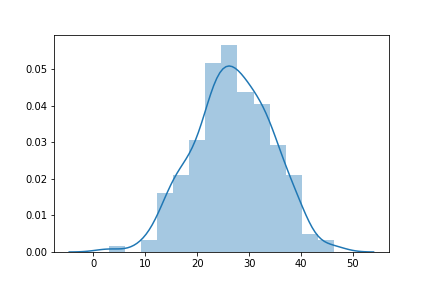
\includegraphics[width=7cm]{Verslag/Tables/Regering.png} }}%
    \subfloat[Tussen twee oppositiepartijen]{{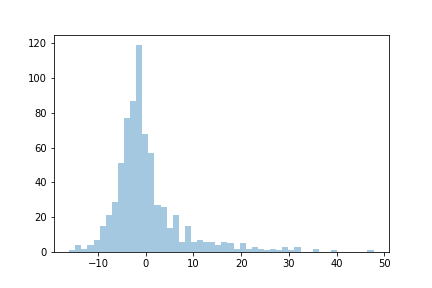
\includegraphics[width=7cm]{Verslag/Tables/Oppositie.png} }}\quad
    \hspace*{-0.2in}
    \subfloat[Tussen een regeringspartij en een oppositiepartij]{{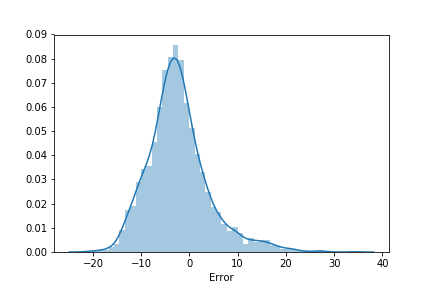
\includegraphics[width=7cm]{Verslag/Tables/Mix.png} }}%
    \subfloat[Totaal]{{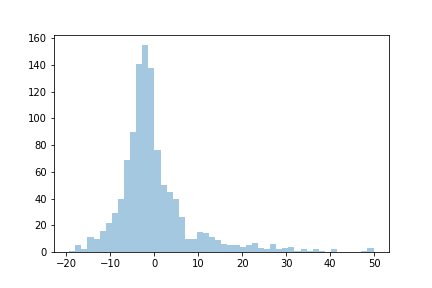
\includegraphics[width=7cm]{Verslag/Tables/Totaal.png} }}\quad
    \caption{Distributie van de error uit formule \ref{eq:error} voor de verschillende combinaties.}%
    \label{fig:distributies}%
\end{figure}

\begin{table}[H] 
\caption{Meest karakteristieke woorden per partij op basis van classificatie uit deelvraag 2 gedurende kabinet-Balkenende IV.} 
\label{tab:WoordenBalkenende4} 
\centering
\hspace*{-1in}
\begin{tabular}{lllll}
\toprule
                  CDA &        ChristenUnie &              D66 &          GroenLinks &         PVV \\
\midrule
       PARTIJ fractie &  fractie van PARTIJ &          premier &       PARTIJfractie &     burgers \\
                  wij &      de fractie van &       de premier &  fractie van PARTIJ &        onze \\
              fractie &          de fractie &          ik hoop &          de fractie &        niet \\
           wij hebben &         fractie van &     arbeidsmarkt &      de fractie van &        deze \\
             KAMERLID &        mijn fractie &  de arbeidsmarkt &         fractie van &  immigratie \\
                 dank &             geweest &             hoop &           politieke &  natuurlijk \\
 PARTIJ fractie heeft &              moment &              hij &             premier &     politie \\
          zorgvuldige &             termijn &   schone energie &                deal &  de burgers \\
                  ons &       verschillende &          plannen &                  ik &      burger \\
         buitengewoon &       beantwoording &           kunnen &                  en &        door \\
\bottomrule
\end{tabular}
 
\end{table} 
\addtocounter{table}{-1} 
\begin{table}[H] 
\caption{Meest karakteristieke woorden per partij op basis van classificatie uit deelvraag 2 gedurende kabinet-Balkenende IV. \emph{(Vervolg)}} 
\centering
\hspace*{-0.6in}
\begin{tabular}{lllll}
\toprule
         PvdA &              PvdD &                    SGP &            SP &             VVD \\
\midrule
          wij &            dieren &           mijn fractie &          zegt &          PARTIJ \\
   belangrijk &     dierenwelzijn &          beantwoording &    leerlingen &    onze fractie \\
      vrouwen &     bio industrie &                    wel &        mensen &  PARTIJ fractie \\
         alle &            natuur &          de voorzitter &            is &         fractie \\
          ben &  de bio industrie &       de voorzitter ik &          niet &              je \\
  volgens mij &            de bio &             natuurlijk &       vandaar &     ondernemers \\
           of &               bio &                diverse &  bureaucratie &            awbz \\
 mijn collega &       dierproeven &               allerlei &            nu &           markt \\
   antwoorden &       veehouderij &      voorzitter ik wil &   voorstellen &          praten \\
         punt &         industrie &  mevrouw de voorzitter &       leraren &      timmermans \\
\bottomrule
\end{tabular}
 
\end{table}

\begin{table}[H]
\caption{Balkenende to Rutte}
\label{tab:baltorut}
\centering
\begin{tabular}{lrrrr}
\toprule
{} &  Precision &  Recall &  F1 score &  Documenten \\
\midrule
CDA          &       0.20 &    0.40 &      0.27 &        1901 \\
ChristenUnie &       0.24 &    0.12 &      0.16 &        1068 \\
D66          &       0.26 &    0.10 &      0.15 &        1889 \\
GroenLinks   &       0.16 &    0.07 &      0.10 &        1068 \\
PVV          &       0.51 &    0.52 &      0.51 &        1700 \\
PvdA         &       0.27 &    0.26 &      0.26 &        1821 \\
PvdD         &       0.72 &    0.19 &      0.31 &         432 \\
SGP          &       0.48 &    0.43 &      0.45 &         655 \\
SP           &       0.35 &    0.59 &      0.43 &        2284 \\
VVD          &       0.21 &    0.10 &      0.14 &        1694 \\
Totaal       &       0.30 &    0.30 &      0.28 &       14512 \\
\bottomrule
\end{tabular}

\end{table}

\begin{table}[H]
\caption{Rutte to Balkenende}
\label{tab:ruttobal}
\centering
\begin{tabular}{lrrrrr}
\toprule
{} &  Precision &  Recall &  \$F\_1\$ score &  Accuracy &  Documenten \\
\midrule
CDA          &       0.29 &    0.30 &         0.29 &       NaN &        1039 \\
ChristenUnie &       0.45 &    0.17 &         0.24 &       NaN &         561 \\
D66          &       0.16 &    0.37 &         0.22 &       NaN &         518 \\
GroenLinks   &       0.33 &    0.03 &         0.05 &       NaN &         760 \\
PVV          &       0.55 &    0.53 &         0.54 &       NaN &         971 \\
PvdA         &       0.27 &    0.28 &         0.27 &       NaN &         903 \\
PvdD         &       0.64 &    0.51 &         0.57 &       NaN &         165 \\
SGP          &       0.54 &    0.56 &         0.55 &       NaN &         507 \\
SP           &       0.42 &    0.52 &         0.46 &       NaN &        1222 \\
VVD          &       0.19 &    0.19 &         0.19 &       NaN &        1041 \\
Totaal       &       0.36 &    0.34 &         0.32 &  0.335501 &        7687 \\
\bottomrule
\end{tabular}

\end{table}

\subsubsection{DV4: Links of rechts}

\subsubsection{DV5: Woordgebruik van sprekers}
In tabel \ref{tab:rapporttaalgebruik} staan de scores van classificatie waarbij de Kamerleden verdeeld zijn over de training en test set. De scores zijn hierbij amper hoger dan de baseline.
\begin{table}[H]
\caption{Classificatierapport van beste classificatie met de Kamerleden verdeeld over training en test set.}
\label{tab:rapporttaalgebruik}
\centering
\begin{tabular}{lrrrr}
\toprule
{} &  Precision &  Recall &  F1 score &  Documenten \\
\midrule
50PLUS       &       0.21 &    0.13 &      0.10 &          33 \\
CDA          &       0.16 &    0.10 &      0.12 &         451 \\
ChristenUnie &       0.09 &    0.05 &      0.06 &         170 \\
D66          &       0.15 &    0.19 &      0.15 &         286 \\
GroenLinks   &       0.10 &    0.07 &      0.07 &         195 \\
PVV          &       0.29 &    0.55 &      0.28 &         273 \\
PvdA         &       0.19 &    0.21 &      0.19 &         323 \\
PvdD         &       0.29 &    0.10 &      0.15 &          78 \\
SGP          &       0.27 &    0.05 &      0.08 &         199 \\
SP           &       0.27 &    0.29 &      0.26 &         469 \\
VVD          &       0.29 &    0.24 &      0.26 &         399 \\
Totaal       &       0.31 &    0.20 &      0.21 &        2875 \\
\bottomrule
\end{tabular}

\end{table}

\subsection{Discussie}
\subsubsection{DV1: Beste classificatiemethode}
Het onderzoek behaalt resultaten in lijn der verwachting op basis van gerelateerd en daarnaast ruim boven de baseline scores. De lage scores voor de coalitiepartijen steunen de hypothese van een afhankelijkheid van partij-status, zoals besproken wordt in deelvraag 3 Het bijna alleen voorkomen van partijnamen en Kamerleden in de meest karakteristieke woorden per partij in tabel \ref{tab:MostImportantWords} steunt daarnaast het vermoeden dat deze classificatie sterk afhankelijk is van die namen, zoals besproken wordt in deelvraag 2.  \par
Dit onderzoek heeft zich beperkt tot methoden genoemd in vergelijkbare onderzoeken en waarvan de implementatie beschikbaar is in scikit-learn. Een aantal methoden die in gerelateerde literatuur leidden tot goede classificaties zijn daarom niet getest. Ook nieuwe methoden die nog niet gebruikt zijn in een vergelijkbaar onderzoek voor politieke tekst classificatie zijn daarom niet getest. Daarnaast richtte zich dit ook maar op een beperkt aantal parameterwaarden. Voor vervolgonderzoek kan daarom dit onderdeel uitgebreid worden. Het effect van het beperkte aantal maximum iteraties was bij de beste classificatiemethode beperkt.\par
Het onderzoek van Hirst et al. vond dat resultaten afhankelijk kunnen zijn van documentgrootte. Alle documenten in dit onderzoek zijn kleiner dan de grootste documentgrootte uit het onderzoek van Hirst et al. en ook de minimumfrequentie lager ligt dan de kleinste documentgrootte uit dat onderzoek.
Het effect wat zij vinden tussen documentgrootte van 267 en 6666 is een verschil in nauwkeurigheid van 19,8\%. Dit onderzoek vindt inderdaad dat kleinere documenten vaker foutief geclassificeerd worden.
\begin{figure}[H]
  \centering
    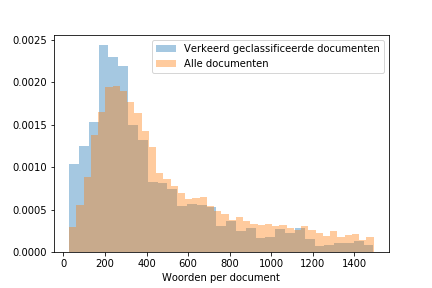
\includegraphics[width=0.40\paperwidth]{Verslag/Tables/misclassifiedlengths.png}
\caption{Genormaliseerde distributie van documentlengtes van foutief geclassificeerde documenten en alle documenten. Totaal van 5-fold cross-validation, waardoor documenten vaker voor kunnen komen.}
\label{fig:misclassified}
\end{figure}
Voor een vervolgonderzoek kan uitgebreider gekeken worden naar dit effect en wat dit betekent voor de resultaten.\par

\subsubsection{DV2: Invloed van namen}
De resultaten laten zien dat de classificatie sterk afhankelijk is van partijnamen en namen van Kamerleden. Deze daling was te verwachten op basis van gerelateerd werk.\par
De woorden in tabel \ref{tab:MostImportantWordsWithoutNames} komen bij veel partijen overeen met hun ideologie, vooral bij PVV, PvdD en 50PLUS. Daarnaast zijn er ook woorden die niet veel over ideologie zeggen, zoals; \textit{volgens mij}, \textit{ik constateer} en \textit{in elk geval}. Vooral de SGP heeft woorden die niet veel lijken te zeggen over de ideologie, hoewel deze partij desalniettemin de hoogste $f_1$ score heeft. Met name opvallend hierbij is \textit{mevrouw de voorzitter}, aangezien deze woorden door alle partijen gebruikt worden om via de voorzitter te praten. Voor een vervolgonderzoek kan gekeken naar waarom deze woorden zo karakteristiek zijn voor partijen. Een hypothese is dat deze woorden eigen zijn aan een individueel Kamerlid.\par
De classificatiemethode die gebruikt is in deze deelvraag, is gebaseerd op de beste methode voor de dataset uit deelvraag 1. Hierin was gevonden dat een combinatie van uni-, bi- en trigrams het beste resultaat opleverde. In tabel \ref{tab:MostImportantWords} is te zien dat trigrams behoren tot de meest karakteristieke woorden, hoewel de woorden in trigrams vaak overlappen met uni- en bigrams. In tabel \ref{tab:MostImportantWordsWithoutNames} daarentegen zijn er nog maar een paar trigrams, welke grotendeels procedurele zinnen zijn of toevoeging van een lidwoord op een uni- of bigram. Dit verschil suggereert dat trigrams minder belangrijk zijn in de classificatie zonder de namen, dus de classificatiemethode uit deelvraag 1 niet het beste is voor deze classificatie. In vervolgonderzoek kan de opzet van deelvraag 1 toegepast worden op de classificatie zonder de namen, om zo te komen tot een classificatiemethode die het beste resultaat oplevert op de classificatie zonder namen.\par 

\subsubsection{DV3: Oppositie of regering}
In tabel \ref{tab:classrapport} is het opvallend dat de coalitiepartijen lage scores krijgt. Daarnaast laat figuur \ref{fig:confusionmatrix} zien dat er een hoge overlap zit tussen deze twee partijen.\par
De resultaten 
De overlap van 100 meest karakteristieke woorden tussen regeringspartijen die niet voorkomen bij oppositiepartijen gedurende kabinet-Rutte II beperkt zich tot de woorden \textit{en} en \textit{blij}, als ook \textit{toezegging} voor VVD en \textit{toezeggingen} voor PvdA.\par
\begin{table}[H]
\label{tab:overlapkabinetten}
\caption{Woorden die bij minimaal één regeringspartij in beide kabinetten voorkomen in de 100 meest karakteristieke woorden, maar niet toen deze partijen in oppositie zaten.}
\centering
\begin{tabular}{|l|l|l|}
\toprule
      &   PvdA &    VVD\\
\midrule
         CDA &    \makecell[l]{toezeggingen\\hun\\collega KAMERLID\\in\\aanpak\\collega} &            \makecell[l]{algemeen\\algemeen overleg\\toezegging\\helder\\overleg\\aangegeven\\voor\\voor PARTIJ} \\ \hline
 ChristenUnie &  \makecell[l]{mijn\\waarop\\blij\\collega KAMERLID\\erg} &        \makecell[l]{gaan\\termijn\\blij met de\\volgens\\volgens mij\\blij\\beantwoording}  \\ \hline
  PvdA &   & \makecell[l]{volgens\\volgens mij}            \\
\bottomrule
\end{tabular}
\end{table}
Hoewel er een aantal overeenkomsten zijn qua meest karakteristieke woorden tussen regeringspartijen, lijkt dit beperkt. De meeste overeenkomsten lijken daarnaast niet heel inhoudelijk gerelateerd aan partij-status. Voor een vervolgonderzoek kan uitgebreider gekeken worden naar de meest karakteristieke woorden en wat deze zeggen over een partij.\par

\subsubsection{DV4: Links of rechts}
Er zijn verschillende visies op links en rechts, en de indeling van de partijen, ook buiten de twee methoden gekozen in dit onderzoek.\par

\subsubsection{DV5: Woordgebruik van sprekers}
De resultaten uit tabel \ref{tab:rapporttaalgebruik} zijn laag, amper hoger dan de baseline. Dit suggereert inderdaad dat eerdere classificaties in grote mate toch afhankelijk waren van het woordgebruik van sprekers. Dit is opmerkelijk aangezien vergelijkbare werken dit effect niet vinden. De meest karakteristieke woorden van deze classificatie wijken daarnaast grotendeels niet af van die uit tabel \ref{tab:MostImportantWordsWithoutNames}.\par
Een alternatieve verklaring is dat de classificatie nu mede op basis van woordvoerderschap is. Per onderwerp heeft een partij vaak maar één woordvoerder, met uitzonderingen van wijzigingen in de fractie. Het is aannemelijk dat het taalgebruik afhankelijk is van woordvoerderschap, aangezien er andere termen gebruikt worden bij bijvoorbeeld een debat over zorg dan bij een debat over onderwijs. Stel dat documenten van een spreker in de test set geclassificeerd moeten worden, dan kan het zijn dat deze meer karakteristieke vertoont met een andere partij, aangezien er geen woordvoerder van die partij en dat onderwerp in de training set zit, maar mogelijk wel van een andere partij. Een vervolgonderzoek kan kijken of dit een verklaring is. \par

\subsubsection{Algemeen}
Het vergelijken van deze resultaten met vergelijkbaar werk is problematisch, aangezien de keuzes en eigenschappen van hun onderzoek het niet een één-op-één vergelijking maken. Voorbeelden hiervan zijn de documentgrootte, baselines, behouden of weglaten van namen, een spreker als document zien en het trainen en testen op dezelfde spreker. Hoewel de resultaten dus lager zijn dan die uit vergelijkbaar werk, moet hiermee rekening gehouden worden. Een vervolgonderzoek zou daarom dit onderzoek kunnen reproduceren op een ander parlement om daarmee te kunnen vergelijken.\par
Dit onderzoek richtte zich hoofdzakelijk op de Handelingen gedurende kabinet-Rutte II. Om te kijken in hoeverre het mogelijk is om deze conclusie door te trekken naar de algemene Handelingen van de Tweede Kamer, kan er in vervolgonderzoek gekeken worden naar meerdere zittingsperioden. Ook kan gekeken worden naar veranderingen als een kabinet demissionair is.\par